\documentclass[twosided,a4paper]{article}           %type
\usepackage[top=2cm,bottom=2cm,inner=1.5cm,outer=1.5cm]{geometry}       %geometry
\renewcommand{\familydefault}{\sfdefault}


%\usepackage[italian]{babel}                %font/language
\usepackage[T1]{fontenc}
\usepackage[utf8]{inputenc}

\usepackage{amsmath}                       %maths
\usepackage{bm}
\usepackage{amssymb}					   %for numbersets

\usepackage{graphicx}
\usepackage{epstopdf} 
\usepackage{float}
\usepackage{subfigure}

\usepackage{tabularx}

%\usepackage{hyperref}

%\usepackage{subfloat}
%full packaging for image in eps finally
\usepackage{textcomp}

\usepackage{color}
\usepackage[dvipsnames]{xcolor}

\usepackage{listings} 

\newcommand{\tr}{^{\tiny{\bm \top}}}

\newenvironment{sistema}%
{\left\lbrace\begin{array}{@{}l@{}}}%
	{\end{array}\right.}

\begin{document}
	
	\title{\textcolor{MidnightBlue}{Mechanical vibration} - \textcolor{Plum}{System identification and modal analysis of 3-DOF linear system}}
	\author{Giammarco Valenti}
	\maketitle
	
\section{Dynamical system}

\subsection{The linear model}
The chosen model is a linear plant consisting of 3 masses, 3 springs between them, and 3 dampers between each mass and the ground. The model is shown in Figure \ref{fig:theplant1}.
\begin{figure}[H]
	\centering
	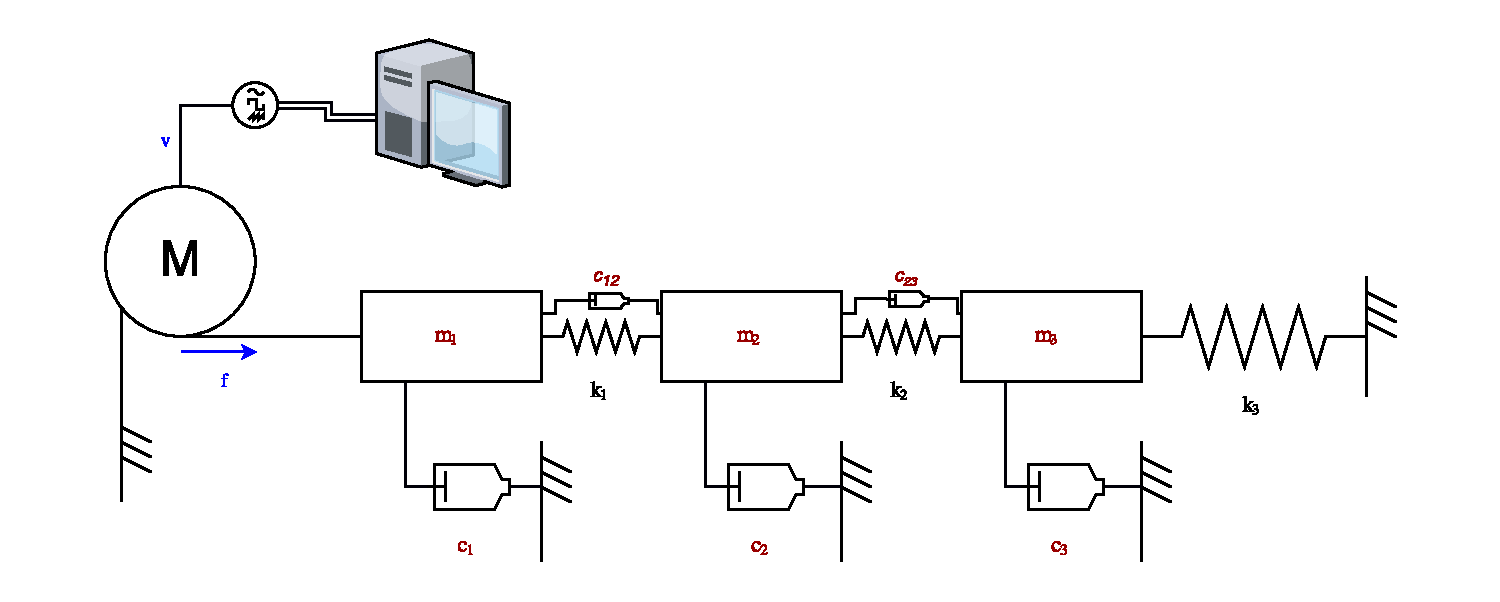
\includegraphics[width=\linewidth]{img/theplant1}
	\caption[The linear plant]{The chosen plant, in red the unknown parameters}
	\label{fig:theplant1}
\end{figure} %TODO figure with displacements x
\subsection{equation of motion}
\begin{equation}
	\begin{sistema}
	m_1 \ddot{x}_1 = + k_1 \left (x_2 - x_1 \right )                                 + c_{12} \left ( \dot{x}_2 - \dot{x}_1 \right )                                                  - c_1\dot{x}_1 + k_v v\\
	m_2 \ddot{x}_2 = + k_1 \left (x_1 - x_2 \right ) + k_2 \left (x_3 - x_2 \right ) + c_{12} \left ( \dot{x}_1 - \dot{x}_2 \right ) +  c_{23} \left ( \dot{x}_3 - \dot{x}_2 \right ) - c_2\dot{x}_2\\
	m_3 \ddot{x}_3 =                                 + k_2 \left (x_2 - x_3 \right )                                                 +  c_{23} \left ( \dot{x}_2 - \dot{x}_3 \right ) - c_3\dot{x}_3 - k_3 x_3
	\end{sistema}
\end{equation}
In the classical matrix form:
\begin{equation}
	\bm M \ddot{x} + \bm C \dot{x} + K \dot{x} = \left [ \ f \ 0\  0 \ \right ]\tr
\end{equation}
where:\\
\begin{subequations}
\noindent\begin{tabularx}{\textwidth}{@{}XXX@{}}
	\begin{equation}
	K = cacca
	\end{equation} &
	\begin{equation}
	C = dampers
	\end{equation} &
	\begin{equation}
	\bm M = \left [\begin{array}{ccc}
	m_1 & 0 & 0 \\ 
	0 & m_2 & 0 \\ 
	0 & 0 & m_3
	\end{array} \right ]
	\end{equation}
\end{tabularx}
\end{subequations}
\subsection{experimental setup}

\subsection{parameters and data available}

\subsection{initial hypothesis and approximations}
\begin{itemize}
	\item rectilinear motion (all perfect aligned)
	\item inerta and damping of the motor are merged respectvely into $m_1$ and $c_1$.
	\begin{equation}
	\begin{sistema}
		m_1 = m_{block} + \frac{J_{motor}\vert_{zz}}{r^2}\\
		c_2 = c_{block} + \frac{c_{motor}}{r^2}
	\end{sistema}
	\end{equation}
	where $r$ is the radius of the gear-rack coupling (gear wheel), $J_{motor}\vert_{zz}$ is the inertia of the motor , $c_{motor}$ the rotational damping and ''block'' quantities are the ones stricly related to the physical first mass.
\end{itemize}
\section{System identification}
	
\subsection{step response analysis}
First of all, the step response analysis can be performed. In this analysis the ''static'' coefficients can be estimated, they are:
\begin{itemize}
	\item voltage to force $k_v$
	\item springs' stiffness $k_i$ with $i \in 1,2,3$
\end{itemize} 
The coefficient to be estimated is the \textcolor{Plum}{\textit{voltage-to-force}} coefficient %TODO SYMBOL 
\begin{equation}
	f = \textcolor{Plum}{\bm{(k_a\cdot k_t \cdot k_{mp})}}v = \textcolor{Plum}{k_v} v
\end{equation}
\subsection{voltage-to-force coefficient estimation}

\subsection{Parameters estimation}

\begin{subequations}
\begin{equation}
	ciao
\end{equation}
\begin{equation}
	ciaone
\end{equation}
\end{subequations}

\end{document}